

\subsection*{Homework Problems}

The following are some more involved problems for you to try, which might be assigned as homework.

\begin{questions}

\question For each sequence given below, find a closed formula for $a_n$, the $n$th term of the sequence (assume the first terms are $a_0$) by relating it to another sequence for which you already know the formula.  In each case, briefly say how you got your answers.  
\begin{parts}
	\part 4, 5, 7, 11, 19, 35, \ldots
	\begin{solution}
		If we subtract 3 from each term, we get $1, 2, 4, 8, 16, 32, \ldots$, which are the powers of 2.  So we must shift this sequence up by 3 to get our sequence.  Thus
		\[a_n = 2^n + 3\]
	\end{solution}
	
	\part 0, 3, 8, 15, 24, 35, \ldots
	\begin{solution}
		Add 1 to each term - we get $1, 4, 9, 16, 25, 36, \ldots$, the square numbers.  So maybe our sequence as formula $a_n = n^2 - 1$.  Does this work?  $a_3 = 8$.  That is a term of our sequence, but it should be $a_2$.  So we want 
		\[a_n = (n+1)^2 - 1\]
	\end{solution}
	
	\part 6, 12, 20, 30, 42, \ldots
	\begin{solution}
		Each term is even, so let's see what happens when we divide by 2: we get $3, 6, 10, 15, 21,\ldots$.  These are the triangle numbers, but starting at $T_2$.  We know $T_n = \frac{n(n+1)}{2}$. We want $a_0 = 2T_2$, $a_1 = 2T_3$, and so on.  In general, $a_n = 2T_{n+2}$, so 
		\[a_n = (n+2)(n+3)\]
		(This is like a shift by 2 units to the left and a stretch by a factor of 2.)
	\end{solution}
	
	\part 0, 2, 7, 15, 26, 40, 57, \ldots (Cryptic Hint: these might be called ``house numbers'')
	\begin{solution}
		How far off from triangular number are these?  The triangular numbers (starting with $T_0$) are $0, 1, 3, 6, 10, 15, 21, \ldots$.  The given sequence differs from this by $0, 1, 4, 9, 16, 25, 36, \ldots$ the square numbers!  Thus
		\[a_n = \frac{n(n+1)}{2} + n^2\]
	\end{solution} 
\end{parts} 

\question Starting with any rectangle, we can create a new, larger rectangle by attaching a square to the longer side.  For example, if we start with a $2\times 5$ rectangle, we would glue on a $5\times 5 $ square, forming a $5 \times 7$ rectangle:

\begin{center}
	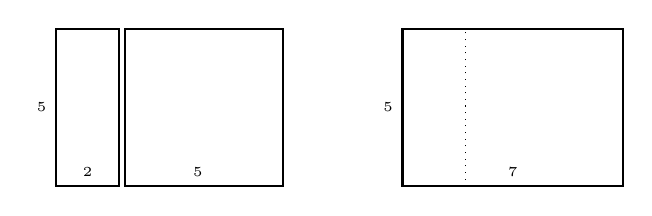
\begin{tikzpicture}[scale=.4]
		\draw[thick] (0,0) rectangle (2,5);
		\draw[thick] (2.2,0) rectangle (7.2,5);
		\draw (0,2.5) node[left]{\tiny 5} (1,0) node[above]{\tiny 2} (4.5,0) node[above]{\tiny 5};
		\draw (9,2.5) node{\Large $\rightsquigarrow$};
		\draw[thick] (11,0) rectangle (18,5);
		\draw[dotted] (13,0) -- (13,5);
		\draw (11,2.5) node[left]{\tiny 5}  (14.5,0) node[above]{\tiny 7};
	\end{tikzpicture}
\end{center}

\begin{parts}
	\part Create a sequence of rectangles using this rule starting with a $1\times 2$ rectangle.  Then write out the sequence of {\em perimeters} for the rectangles (the first term of the sequence would be 6, since the perimeter of a $1\times 2$ rectangle is 6 - the next term would be 10).
	\begin{solution}
		The rectangles are $1 \times 2$, $2 \times 3$, $3 \times 5$, $5 \times 8$, $8 \times 13$, and so on.  The sequence of perimeters is \[6, 10, 16, 26, 42, \ldots\]
	\end{solution}
	
	\part Repeat the above part this time starting with a $1 \times 3$ rectangle.
	\begin{solution}
		The sequence of rectangles have dimensions $1\times 3$, $3 \times 4$, $4 \times 7$, $7 \times 11$, $11\times 18$, and so on.  The sequence of perimeters is \[8, 14, 22, 36, 58, \ldots\]
	\end{solution}
	
	\part Find recursive formulas for each of the sequences of perimeters you found in parts (a) and (b).  Don't forget to give the initial conditions as well.
	\begin{solution}
		For the sequence from (a), the recursive formula is $a_1 = 6$, $a_2 = 10$, and $a_n = a_{n-1} + a_{n-2}$.
		
		For the sequence from (b), the recursive formula is $a_1 = 8$, $a_2 = 14$, and $a_n = a_{n-1} + a_{n-2}$.  
		
		Notice that both sequence have the same rule for getting terms from the previous ones, it is just the initial conditions that are different.  
	\end{solution}
	
	\part Are the sequences arithmetic?  Geometric?  If not, are they {\em close} to being either of these (i.e., are the differences or ratios {\em almost} constant)?  Explain.
	\begin{solution}
		The sequences are not arithmetic because the differences between terms is not constant.  Similarly the ratio between terms is not constant, so the sequences are not geometric either.  
		
		However, look at the ratio between terms: $10/6 \approx 1.66$, $16/10 = 1.6$, $26/16 \approx 1.625$, $42/26 \approx 1.61$, \ldots.  In fact, the ratio between terms of the second sequence also floats around this same number.
		
		That number (and in fact, the limit of the ratios of either sequence as the terms increase) is $\frac{1 + \sqrt{5}}{2} \approx 1.618$, also known as the golden ratio.
		\end{solution}
\end{parts}



\question If you have enough toothpicks, you can make a large triangular grid.  Below, are the triangular grids of size 1 and of size 2.  The size 1 grid requires 3 toothpicks, the size 2 grid requires 9 toothpicks.

\centerline{\includegraphics[height=1in]{images/triangles.png}}

\begin{center}
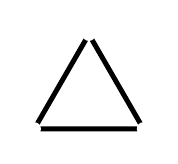
\begin{tikzpicture}[scale=.8]
\draw[line width=1.8pt] (90:1) -- (-30:1) -- (210:1) -- (90:1);
\fill[color=white] (90:1) circle (3pt);
\fill[color=white] (-30:1) circle (3pt);
\fill[color=white] (210:1) circle (3pt);
\end{tikzpicture}
\qquad
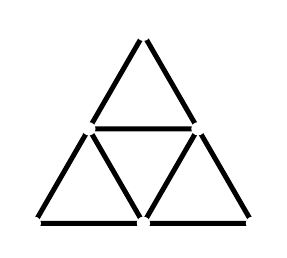
\begin{tikzpicture}[scale=.8]
\draw[line width = 1.8pt] (-90:1) -- (210:2) -- (150:1) -- (-90:1) -- (-30:2) -- (30:1) -- (150:1) -- (90:2) -- (30:1) -- (-90:1);
\fill[color=white] (-90:1) circle (3pt);
\fill[color=white] (-30:2) circle (3pt);
\fill[color=white] (210:2) circle (3pt);
\fill[color=white] (90:2) circle (3pt);
\fill[color=white] (30:1) circle (3pt);
\fill[color=white] (150:1) circle (3pt);
\end{tikzpicture}
\end{center}
 
\begin{parts}
  \part Let $t_n$ be the number of toothpicks required to make a size $n$ triangular grid.  Write out the first 5 terms of the sequence $t_1, t_2, \ldots$.
  \begin{solution}
    $ 3, 9, 18, 30, 45, \ldots$
  \end{solution}

  \part Find a recursive definition for the sequence.  Explain why you are correct.
  \begin{solution}
    $t_n = t_{n-1} + 3n$ with $t_1 = 3$.  This works because to get the next larger triangular grid, we must add a row of $n$ triangles, each requiring 3 toothpicks.
  \end{solution}

  \part Is the sequence arithmetic or geometric?  If not, is it the sequence of partial sums of an arithmetic or geometric sequence?  Explain why your answer is correct.
  
  \begin{solution}
	  The sequence is not arithmetic (since $9-3 = 6$ but $18-9 = 9$).  It is also not geometric (since $9/3 = 3$ but $18/9 = 2$).  To decide whether the sequence is a sequence of partial sums, we look at the differences.  The sequence of differences is $6, 9, 12, 15, \ldots$.  This {\em is} an arithmetic sequence.  So we see that
	  \[t_1 = 3\]
	  \[t_2 = 3+6\]
	  \[t_3 = 3+6+9\]
	  \[t_4 = 3+6+9+12\]
	  \[t_n = \sum_{k = 1}^n 3k\]
  \end{solution}

  \part Use your results from part (c) to find a closed formula for the sequence.  Show your work.
  \begin{solution}
    We have $t_n = 3 + 6 + 9 + \cdots + 3n$.  If we reverse these and add corresponding terms we get
    \[2t_n = (3n+3) + (3n+3) + (3n+3) + \cdots + (3n+3)\]
    On the right hand side of the equation we have the sum of $n$ copies of $(3n+3)$ so we get
    \[2t_n = n(3n+3)\]
    or \[t_n = \frac{n(3n+3)}{2}\]
    
    This is not a huge surprise.  Notice that each term in the sequence is a multiple of 3.  Dividing each term by 3 gives the sequence $1,3, 6, 10, 15,\ldots$ - the triangular numbers. This makes sense because we are forming triangles out of 3-toothpick collections.   So a closed formula is therefore
    $t_n = 3\frac{n(n+1)}{2}$
  \end{solution}

\end{parts}



\question Consider the sequence $5, 11, 19, 29, 41, 55,\ldots$.  Assume $a_1 = 5$.
\begin{parts}
\part Find a closed formula for $a_n$, the $n$th term of the sequence, by writing each term as a sum of a sequence.  Hint: first find $a_0$, but ignore it when collapsing the sum.
\begin{solution}
$a_0 = 1$, $a_1 = 1+4$, $a_2 = 1+4+6$, $a_3 = 1+4+6+8$ and so on.  If we ignore (for the moment) the 1, we have the sum of an arithmetic sequence.  So
\begin{align*}
a_n & = 1 + [4 + 6 + 8 + 10 + \cdots + (2n) + (2+2n)]\\
+ a_n & = 1 + [(2+2n) + (2n) + \cdots +  8 + 6 + 4] \\ \hline
2a_n & = 1 + n(2n+6)
\end{align*}

So $a_n = \frac{1+n(2n+6)}{2}$
\end{solution}


\part Find a closed formula again, this time using either polynomial fitting or the characteristic root technique (whichever is appropriate).  Show your work.

\begin{solution}
The sequence of first differences is $4, 6, 8, 10, 12,\ldots$, so the sequence of second differences is $2, 2, 2,\ldots$ which is constant.  Thus we know that the original sequence will be a quadratic: $a_n = an^2 + bn + c$.  We know $a_0 = 1$ so we have $c = 1$.  This gives the system
\[5 = a + b + 1\]
\[11 = 4a + 2 b + 1\]
If we multiply the first equation by $-2$ and add the second equation we get $1 = 2a - 1$ so $a = 1$.  Plugging this into the first equation gives $b = 3$.  Thus the closed formula is $a_n = n^2 + 3n + 1$.
\end{solution}

\part Find a closed formula once again, this time by recognizing the sequence as a modification to some well known sequence(s).  Explain.
\begin{solution}
If we compare our sequence to the sequence of squares $1,4,9, 16, 25,\ldots$ we see a difference of $4, 7, 10, 13, 16, \ldots$.  These are each 1 more than a multiple of 3.  So we see that the sequence $5, 11, 19, 29, 41, 55,\ldots$ is just the sequence of squares plus the sequence given by $3n+1$.  So
\[a_n = n^2 + 3n + 1\]

\end{solution}

\end{parts}


\question In their down time, ghost pirates enjoy stacking cannonballs in triangular based pyramids (aka, tetrahedrons), like those pictured here:

%\centerline{\includegraphics[height=1in]{images/cannonballs.png}}

\begin{center}

\begin{tikzpicture}
\def\shadowprops{{fill=black!50,shadow xshift=0.5ex,shadow yshift=0.5ex,path fading={circle with fuzzy edge 10 percent}}}

\draw (0,0) circle (10pt);
\draw[very thin, color=brown!15] (0,0) circle (10pt);
\shade[shading=axis,bottom color=black!70!brown, top color=black!15, shading angle=-40] (0,0) circle (10pt);
\end{tikzpicture}
\qquad

\begin{tikzpicture}
\foreach \pos in {(-.32, .2), (.32,.2), (0,.55), (0,0)}{
\draw[very thin, color=brown!15] \pos circle (10pt);
\shade[shading=axis,bottom color=black!70!brown, top color=black!15, shading angle=-40] \pos circle (10pt);
}
\end{tikzpicture}
\qquad

\begin{tikzpicture}
\foreach \pos in {(-.64, .4), (.64,.4), (-.37, .75), (.37,.75), (0, 1.2), (-.32, .2), (.32,.2), (0,.6), (0,0)}{
\draw[very thin, color=brown!15] \pos circle (10pt);
\shade[shading=axis,bottom color=black!70!brown, top color=black!15, shading angle=-40] \pos circle (10pt);
}
\end{tikzpicture}
\end{center}

Note, in the picture on the right, there are some cannonballs (actually just one) you cannot see. The next picture would have 4 cannonballs you cannot see.  The stacks are \emph{not} hollow. 

The pirates wonder how many cannonballs would be required to build a pyramid 15 layers high (thus breaking the world cannonball stacking record).  Can you help?

\begin{parts}
\part Let $P(n)$ denote the number of cannonballs needed to create a pyramid $n$ layers high.  So $P(1) = 1$, $P(2) = 4$, and so on.  Calculate $P(3)$, $P(4)$ and $P(5)$.
\begin{solution}
  To get the next larger pyramid, we add a triangle of cannonballs to the previous pyramid.  Thus to get $P(n)$, we add $P(n-1)$ to the $n$th triangular number:
  $P(3) = 4 + 6 = 10$, $P(4) = 10 + 10 = 20$, $P(5) = 20 + 15 = 35$.
\end{solution}


\part Use polynomial fitting to find a closed formula for $P(n)$.  Show your work.
\begin{solution}
  The first differences are $3, 6, 10, 15, \ldots$.  The second differences are $3, 4, 5, 6, \ldots$.  The third differences are $1,1,1,\ldots$.  Since third differences are constant, we know the closed formula for $P(n)$ will be a degree 3 polynomial.  So $P(n) = an^3 + b n^2 + cn + d$.  Note that $P(0) = 0$, so $d = 0$.  To solve for $a$, $b$, and $c$, we solve the system of equations:
  \begin{align*}
    1 & = a + b + c \\
    4 & = 8a+ 4b + 2c \\
    10 & = 27a + 9b + 3c
  \end{align*}
  Doing so gives $a = \frac{1}{6}$, $b = \frac{1}{2}$ and $c = \frac{1}{3}$ so 
  \[P(n) = \frac{1}{6}n^3 + \frac{1}{2} n^2 + \frac{1}{3} n\]
\end{solution}


\part Answer the pirate's question: how many cannonballs do they need to make a pyramid 15 layers high?

\begin{solution}
  \[P(15) = \frac{1}{6}15^3 + \frac{1}{2} 15^2 + \frac{1}{3} 15 = 680\]
\end{solution}

\end{parts}


\question Consider the sequences $2, 5, 12, 29, 70, 169, 408,\ldots$ (with $a_0 = 2$).  
\begin{parts}
\part Describe the rate of growth of this sequence.
\begin{solution}
It does not seem to help to look at the difference between terms - in fact, the differences seem to be growing in the same manner as the original sequence.  However, looking at the ratio between terms gives us almost a common ratio of 2.  In other words, it appears that the sequence is growing exponentially.
\end{solution}


\part Find a recursive definition for the sequence.
\begin{solution}
We see that $5$ is a little more than twice the previous term, and 12 is a little more than twice 5.  In fact, it is exactly 2 more, which is the first term.  So perhaps $a_n = 2a_{n-1} + a_{n-2}$, and this seems to work moving forward.
\end{solution}

\part Find a closed formula for the sequence.

\begin{solution}
Use the characteristic root technique.  The characteristic equation is $x^2 - 2x - 1 = 0$.  Solving this (using the quadratic formula) gives $x = 1\pm\sqrt{2}$.  So we know that the closed formula for $a_n = a(1+\sqrt{2})^n + b(1-\sqrt{2})^n$.  Now let's find $a$ and $b$.  We have

\[2 = a + b\]
\[5 = a(1+\sqrt{2}) + b(1-\sqrt{2})\]
Use substitution: $a = 2-b$ so $5 = (2-b)(1+\sqrt 2) + b(1-\sqrt{2})$ which simplifies to $b = \frac{3\sqrt{2} - 4}{4}$.  This gives $a = \frac{4 - 3\sqrt 2}{4}$.  Therefore
\[a_n = \frac{4-3\sqrt{2}}{4}(1+\sqrt{2})^n + \frac{3\sqrt{2} - 4}{4}(1-\sqrt{2})^n\]
\end{solution}

\part If you look at the sequence of differences between terms, and then the sequence of second differences, the sequence of third differences, and so on, will you ever get a constant sequence?  Explain how you know.
\begin{solution}
You will never get a constant sequence of differences.  If you did, this would mean that the original sequence would be some polynomial.  But we have an exponential closed formula, so no polynomial will fit.
\end{solution}
\end{parts}


\question Let $a_n$ be the number of  $1 \times n$ tile designs can you make using $1 \times 1$ squares available in 4 colors and $1 \times 2$ dominoes available in 5 colors.
\begin{parts}
  \part First, find a recurrence relation to describe the problem.  Explain why the recurrence relation is correct (in the context of the problem).
  \begin{solution}
    $a_n = 4a_{n-1} + 5a_{n-2}$.  Each path of length $n$ must either start with one of the 4 $1\times 1$ tiles, in each case there are then $a_{n-1}$ ways to finish the path, or start with one of the 5 $1\times 2$ tiles, in each case there are then $a_{n-2}$ ways to finish the path.
  \end{solution}

  \part Write out the first 6 terms of the sequence $a_1, a_2, \ldots$.
  \begin{solution}
    4, 21, 104, 521, 2604, 13021
  \end{solution}

  \part Solve the recurrence relation.  That is, find a closed formula for $a_n$.
  \begin{solution}
    The characteristic equation is $x^2 - 4x - 5 = 0$ so the characteristic roots are $x = 5$ and $x = -1$.  Therefore the general solution is 
    \[a_n = a 5^n + b (-1)^n\]
    We solve for $a$ and $b$ using the fact that $a_1 = 4$ and $a_2 = 21$.  We get $a = \frac{5}{6}$ and $b = \frac{1}{6}$.  Therefore the solution is
    \[a_n = \frac{5}{6} 5^n + \frac{1}{6}(-1)^n\]
  \end{solution}

\end{parts}






\question Consider the recurrence relation $a_n = 4a_{n-1} - 4a_{n-2}$.
\begin{parts}
  \part Find the general solution to the recurrence relation (beware the repeated root).
  \begin{solution}
    The characteristic polynomial is $x^2 - 4x + 4$ which factors as $(x -2)^2$, so the only characteristic root is $x = 2$.  Thus the general solution is
    \[a_n = a2^n + bn2^n\]
  \end{solution}

  \part Find the solution when $a_0 = 1$ and $a_1 = 2$.
  \begin{solution}
    Since $1 = a2^0 + b\cdot 0 \cdot 2^0$ have have $a = 1$.  Then $2 = 2^1 + b 2^1$ so $b = 0$.  We have the solution 
    \[a_n = 2^n\]
  \end{solution}

  \part Find the solution when $a_0 = 1$ and $a_1 = 8$.
  \begin{solution}
    Again, we have $a = 1$.  Now when we plug in $n = 1$ we bet $8 = 2 + 2b$ so $b = 3$.  The solution:
    \[a_n = 2^n + 3n2^n\]
  \end{solution}

\end{parts}







\question Zombie Euler and Zombie Cauchy, two famous zombie mathematicians, have just signed up for Twitter accounts.  After one day, Zombie Cauchy has more followers than Zombie Euler.  Each day after that, the number of new followers of Zombie Cauchy is exactly the same as the number of new followers of Zombie Euler (and neither lose any followers).  Explain how a proof by mathematical induction can show that on every day after the first day, Zombie Cauchy will have more followers than Zombie Euler.  That is, explain what the base case and inductive case are, and why they together prove that Zombie Cauchy will have more followers on the 4th day.

\begin{solution}
  The idea here is that because we know Zombie Cauchy starts ahead, and each day increases by the same amount as Zombie Euler, he will always be ahead.
  
   The base case is that Zombie Cauchy has more followers than Zombie Euler on day 1.  We know this is true because it says so in the problem.
    
    The inductive case is that {\em if} Zombie Cauchy has more followers on day $k$, then he will still have more followers on day $k+1$.  We know this is true because each day, the Zombies receive an equal number of new followers. 
    
    Together, the base case and inductive case show that on the 4th day, Zombie Cauchy will be ahead: he is ahead on day 1, and because on day 1 he is ahead, by the inductive case he will also be ahead on day 2.  By the inductive case again, he will be ahead on day 3 since he is ahead on day 2, and since he is ahead on day 3, he will also be ahead on day 4.  Of course we could keep doing this up to any day.
\end{solution}

%\uplevel{{\bf Special Induction Instructions}: For the rest of the homework problems, you should first give a rough sketch of the argument (i.e., say {\em why} induction will work in this case) and then also give a formal proof by induction (starting with, ``Let $P(n)$ be the statement\ldots'').}

\question Find the largest number of points which a football team cannot get exactly using just 3-point field goals and 7-point touchdowns (ignore the possibilities of safeties, missed extra points, and two point conversions).  Prove your answer is correct by mathematical induction.

\begin{solution}
  First note that it is impossible to make 11 points - if only field goals are made, the points must be a multiple of 3, if 1 touchdown is made, the possible point totals are 7, 10, 13, \ldots and two touchdowns are already too much.
  
  We will prove that 11 is the largest number of points which cannot be made.  In other words, any number of points greater than or equal to 12 can be made.
  
  \begin{proof}
    Let $P(n)$ be the statement ``it is possible to make $n$ points using touchdowns and field goals.''  We will prove $P(n)$ is true for all $n \ge 12$.
    
    First the base case: You can make 12 points with 4 field goals, so $P(12)$ is true.
    
    Now the inductive case: Assume $P(k)$ is true for some fixed $k \ge 12$.  That is, it is possible to make $k$ points.  Since $k \ge 12$, we must have made the $k$ points using either at least 2 field goals or at least 2 touchdowns, or both (because if we used just one of each we would have only 10 points).  Now if the $k$ points were accomplished with 2 (or more) field goals, then replace 2 field goals with 1 touchdown.  This increases to point total by 1, giving $k + 1$ points.  On the other hand, if the $k$ points were accomplished with $2$ (or more) touchdowns, replace 2 touchdowns with 5 field goals, again increasing the point total by 1, giving $k+1$ points.  Using one of these two substitutions, we can make $k+1$ points, so $P(k+1)$ is true, establishing the inductive case.
    
    Therefore by the principle of mathematical induction, $P(n)$ is true for all $n \ge 12$.
  \end{proof}
\end{solution}

\question Prove that the sum of $n$ squares can be found as follows\[1^2 +2^2 +3^2+...+n^2 = \frac{n(n+1)(2n+1)}{6}\]
\begin{solution}
This question is asking us to show that the sum of squares for $n$ numbers can be found using the formula $\frac{n(n+1)(2n+1)}{6}$. We can definitely see this is true for the first few instances, but we are really taking it on faith that it is true for the first $n$ squares. So, it seems like induction would be a good place to start.
\begin{proof}
First, let $P(n)$ be the statement that is given.

Base case: We must now show that our base case $P(1)$ is true \[1^2 = \frac{1(1+1)(2(1)+1)}{6} = \frac{6}{6} =1\]

Inductive case: Now, we assume that for some $k\leq n$ that $P(k)$ is true and show that $P(k+1)$ is true. Namely, assume that $1^2 +2^2 +3^2+...+k^2 = \frac{k(k+1)(2k+1)}{6}$ and show that \[1^2 +2^2 +3^2+...+k^2+{(k+1)}^2 = \frac{(k+1)((k+1)+1)(2(k+1)+1)}{6}\]

At this point it is advantageous to start on one side of the equality. So, choosing the left hand side to start I shall manipulate it so that it looks like the right hand side.

\begin{align*}
1^2 +2^2 +3^2+...+k^2+{(k+1)}^2 = \\
= & \frac{k(k+1)(2k+1)}{6} +(k+1)^2 \mbox{ by our inductive hypothesis}\\
= & \frac{k(k+1)(2k+1)}{6} +\frac{6(k+1)^2}{6} \\
= & \frac{k(k+1)(2k+1)+6(k+1)^2}{6} \\
= & \frac{(k+1)[k(2k+1)+6(k+1)]}{6} \mbox{ factoring out $k+1$ from each term}\\
= & \frac{(k+1)[2k^2+k+6k+6]}{6}\\
= & \frac{(k+1)[2k^2+7k+6]}{6}\\
= & \frac{(k+1)[(2k+3)(k+2)]}{6}\\
= & \frac{(k+1)(2(k+1)+1)((k+1)+1)}{6}
\end{align*}
Thus, $P(k+1)$ is true.

Therefore, by the principle of mathematical induction $P(n)$ is true for all $n \geq 1$ 
\end{proof}
\end{solution}
\question  Prove, by mathematical induction, that $F_0 + F_1 + F_2 + \cdots + F_{n} = F_{n+2} - 1$, where $F_n$ is the $n$th Fibonacci number ($F_0 = 0$, $F_1 = 1$ and $F_n = F_{n-1} + F_{n-2}$).
\begin{solution}
This is saying that if we add up the first $n$ Fibonacci numbers, we will get another Fibonacci number (specifically, the $(n+2)$th one).  Induction is a good idea here because it will be easy to just add one more Fibonacci number to the sum we already have.  If we already have $F_{k+2}$ and we add $F_{k+1}$ we can use the recurrence relation to simplify this, becoming $F_{k+3}$.  
 
  \begin{proof}
    Let $P(n)$ be the statement $F_0 + F_1 + F_2 + \cdots + F_n = F_{n+2} - 1$.  We will prove that $P(n)$ is true for all $n \ge 0$.  
    
    Base case: $P(0)$ states that $F_0 = F_2 - 1$, which is true because $F_0 = 0$ and $F_2 = 1$.
    
    Inductive case:  Assume $P(k)$ is true for an arbitrary fixed $k \ge 0$.  That is, \[F_0 + F_1 + F_2 + \cdots + F_k = F_{k+2} - 1\]
    We must prove that $P(k+1)$ is true as well (i.e. that $F_0 + F_1 + \cdots +F_{k+1} = F_{k+3} - 1$).  Start with the left hand side:
    \begin{align*}
      F_0 + F_1 + F_2 + \cdots + F_k + F_{k+1} & = F_{k+2} - 1 + F_{k+1} & \mbox{ by the inductive hypothesis}\\
      & = F_{k+3} - 1 & \mbox{ by the definition of the Fibonacci numbers}
    \end{align*}
    Thus $P(k+1)$ is true.
    
    Therefore by the principle of mathematical induction, $P(n)$ is true for all $n \ge 0$.
  \end{proof}

\end{solution}



\question Prove, using strong induction, that every natural number is either a Fibonacci number or can be written as the \emph{sum} of \emph{distinct} Fibonacci numbers.

	\begin{solution}
		\begin{proof}
			Let $P(n)$ be the statement ``$n$ is either a Fibonacci number or is the sum of distinct Fibonacci numbers.''  We will prove $P(n)$ is true for all $n \ge 0$.  Note that $P(0)$, $P(1)$, $P(2)$, and $P(3)$ are all true since $0, 1, 2, 3$ are Fibonacci numbers.  
			
			Suppose that $P(k)$ is true for all $k < n$.  Now if $n$ is a Fibonacci number, then $P(n)$ is true.  Otherwise, let $m$ be the largest Fibonacci number less than $n$.  Consider the number $n - m$.  This is a number smaller than $n$, so $P(n-m)$ is true.  So wrote $n-m$ either as a single Fibonacci number (if it is one) or as the sum of distinct Fibonacci numbers.  Adding the Fibonacci number $m$ will give $n$ as the sum of Fibonacci numbers.  All that is left is to explain why this sum does not have any repeats (that the numbers are distinct).  We know that there are no repeats in the sum for $n-m$ by the inductive hypothesis.  So the only way we might get a repeat is if the sum for $n-m$ contained an $m$.  But there must be a Fibonacci number between $m$ and $2m$ (since $m$ plus the previous Fibonacci number is a Fibonacci number), and we picked $m$ to be the largest Fibonacci number less than $n$.  This would mean that $2m > n$, so there cannot be two $m$'s in the sum.
		\end{proof}
	\end{solution}

% This is an example in the notes.  Maybe do the Fibonacci numbers one?
%\question Prove that for any integer $n\geq 2$, $n$ is either prime or a product of primes. Use strong induction.  Hint: If $n > 2$ and is \textbf{not} prime, then $n = a\cdot b$ where $a$ and $b$ are less than $n$.
%
%\begin{solution}
%This question is asking us to prove that every integer is a product of primes. That is, we are basically showing the existence of the prime factorization for every integer. Since the question asks us to use strong induction, we are going to first show a base case is true and then assume that if $P(k)$ with $k\geq 2$ and $k<n$ is true then $P(n)$ is also true.
%\begin{proof}
%Let $P(n)$ be the statement ``for any integer $n\geq 2$, $n$ is either a prime or a product of primes''
%
%Base case: $P(2)$ is then our first case (because $n\geq 2$) and $P(2)$ states that $n=2$ is either a prime or a product of primes. Well, $2$ is in fact a prime number. So, our base case is satisfied.
%
%Inductive case: Assume that for all $k\geq 2$ and $k<n$ that $P(k)$ is true. Namely, $k$ is either a prime or a product of primes. Now, since we are using strong induction, we need to show that $P(n)$ holds. That is, we need to show that $n$ is either prime or a product of primes. If $n$ is a prime, then we are done. So, assume that $n$ is not prime. Then we need to show that $n$ can be written as a product of primes. Since $n$ is not a prime, $n=ab$ where $a,b$ are two integers such that $2 \leq a, b<n$. Now, if $a=2$ then the largest possible value for $b$ is $\frac{n}{2}$, so $a,b< \frac{n}{2} <k$. Therefore by our inductive case, $a$ and $b$ are both either a prime or a product of primes. Namely,
%
%\[a=p_1p_2\cdots p_i \text{ where each $p_i$ is a prime or } a \text{ is prime} \] 
%\[b=r_1r_2\cdots r_j \text{ where each $r_j$ is a prime or } b \text{ is prime}\]
%Thus, $k+1=ab$ is a product of primes.
%
%Therefore by the strong induction principle $P(n)$ is true for all $n\geq 2$
% \end{proof}
% \end{solution}
 
 

 
\end{questions}


